\pgfplotsset{
	axis lines=middle,
	axis line style={->},
	xmin=0,
	xticklabels=empty,
	xtick=\empty,
	ymin=-1,
	ymax=1,
	yticklabels=empty,
	ytick=\empty,
	samples=200,
	every axis plot post/.append style={very thick},
	every axis x label/.append style={at={(1.25,0.7)}},
	clip=true,
}% end of common axis set
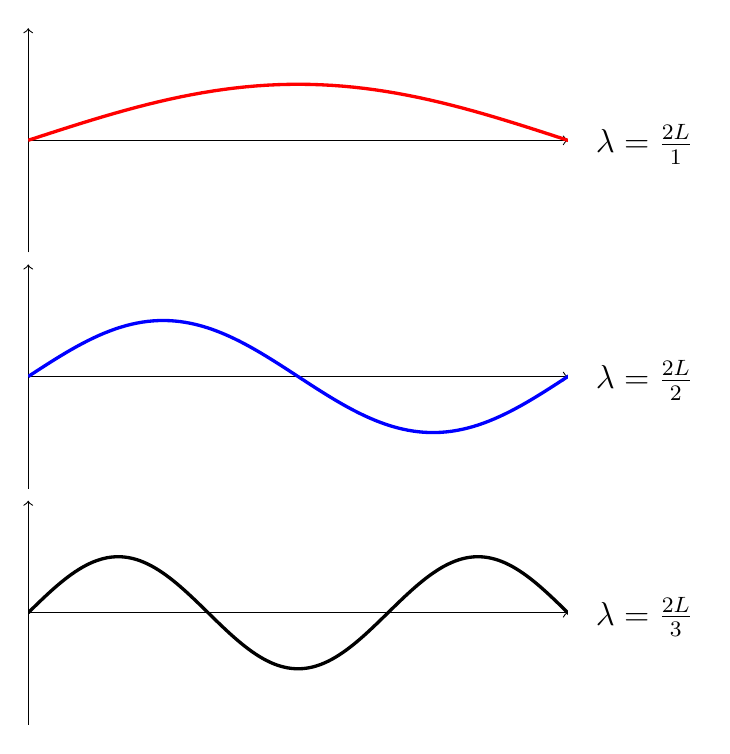
\begin{tikzpicture}
	\begin{axis}% 1. plot
		[
		domain=0:4*pi,
		xmax=pi,
		yscale=0.5,
		xlabel={\large$\lambda=\frac{2L}{1}$}
		]
		\addplot[red] {(sin(deg(x+pi))/2)*-1};
	\end{axis}
	\begin{axis}% 2. plot
		[
		domain=0:4*pi,
		xmax=2*pi,
		yshift=-3cm,
		yscale=0.5,
		xlabel={\large$\lambda=\frac{2L}{2}$}
		]
		\addplot[blue] {(sin(deg(x+pi))/2)*-1};
	\end{axis}
	\begin{axis}% 3. plot
		[
		domain=0:4*pi,
		xmax=3*pi,
		yshift=-6cm,
		yscale=0.5,
		xlabel={\large$\lambda=\frac{2L}{3}$}
		]
		\addplot[black] {(sin(deg(x+pi))/2)*-1};
	\end{axis}
\end{tikzpicture}
